\documentclass[8pt]{beamer}

\usetheme[numbering=fraction, progressbar=foot, block=fill]{metropolis}

\makeatletter
\setlength{\metropolis@titleseparator@linewidth}{1pt}
\setlength{\metropolis@progressonsectionpage@linewidth}{2pt}
\setlength{\metropolis@progressinheadfoot@linewidth}{2pt}
\makeatother

\usepackage{appendixnumberbeamer}
\usepackage{booktabs}
\usepackage{pgfplots}
\usepackage{tikz}
\usepackage{multicol}
\usepackage{changepage}
\usepackage{hyperref}
\usepackage{multirow}
\usepackage{arydshln}
\usepackage[document]{ragged2e}
\usepgfplotslibrary{dateplot}
\usepackage{xspace}

\newcommand{\themename}{\textbf{\textsc{metropolis}}\xspace}

% ================== Customization
\definecolor{mygreen}{RGB}{40,85,175} %Dark green
\definecolor{myred}{RGB}{153,26,0} %Dark red
\definecolor{myblue}{RGB}{66,98,163} %Dark blue
\definecolor{mycolor}{RGB}{66,98,163}

\setbeamercolor{background canvas}{bg=white}

%\setbeamertemplate{blocks}[rounded][shadow=false]

% ================== Title page
\title{Search for dark matter production in association with top quarks in the dilepton final state at $\sqrt{s} = $ 13 TeV}
%\subtitle{The subtitle goes here}
%\date{\today}\newcommand{\themename}{\textbf{\textsc{metropolis}}\xspace}

% ================== Customization
\definecolor{mygreen}{RGB}{40,85,175} %Dark green
\definecolor{myred}{RGB}{153,26,0} %Dark red
\definecolor{myblue}{RGB}{66,98,163} %Dark blue
\definecolor{mycolor}{RGB}{66,98,163}

\setbeamercolor{background canvas}{bg=white}

%\setbeamerfont{institute}{series=\bfseries,parent=structure}
\setbeamerfont{institute}{size=\large}
\setbeamerfont{author}{size=\normalsize}
\setbeamerfont{date}{size=\normalsize}

\newcommand{\backupbegin}{
   \newcounter{finalframe}
   \setcounter{finalframe}{\value{framenumber}}
}
\newcommand{\backupend}{
   \setcounter{framenumber}{\value{finalframe}}
}

%\setbeamertemplate{blocks}[rounded][shadow=false]

%\subtitle{The subtitle goes here}
%\date{\today}
%\date{}
%\author{\justifying Afiq Anuar, Alexander Grohsjean, Christian Schwanenberger, Dominic Stafford, Nicole Stefanov (1), Kristian Hahn, Kevin Sung (2), Pablo Martinez Ruiz Del Arbol, J\'{o}natan Piedra,  \textbf{C\'{e}dric Prieels (3)}, Deborah Pinna, Victor Shang (4)}
%\institute{\textbf{\textbf{January 8th 2021}} \\ 
%\begin{multicols}{2}
%\normalsize{(1) DESY} \\
%(2) NorthWestern University \\
%(3) Instituto de Fisica de Cantabria \\
%(4) University of Wisconsin
%\end{multicols}}
%
%\titlegraphic{
%   \tikz[overlay,remember picture]
%       \node[at=(current page.south east), anchor=south east] {
%           
\includegraphics[height=1cm]{figs/desy.png}\hspace{18pt}
\includegraphics[height=1.1cm]{figs/northwestern.png}\hspace{18pt}
\includegraphics[height=0.9cm]{figs/ifca.jpg}\hspace{18pt}
\includegraphics[height=1cm]{figs/wisconsin.png}\hspace{18pt}
\includegraphics[height=1cm]{figs/cms.jpg}
%       };
%}

\date{\vspace{-3pt}February 22th 2021}
\author{Pablo Mart\'{i}nez Ru\'{i}z del \'{A}rbol, J\'{o}natan Piedra Gomez, \textbf{C\'{e}dric Prieels}}
\institute{Instituto de F\'{i}sica de Cantabria}

\titlegraphic{
   \tikz[overlay,remember picture]
       \node[at=(current page.south east), anchor=south east] {
           
\includegraphics[height=1.0cm]{figs/ifca_final.png}\hspace{18pt}
\includegraphics[height=1.2cm]{figs/uc.jpg}\hspace{8pt}
\includegraphics[height=1.4cm]{figs/csic.jpg}\hspace{8pt}
\includegraphics[height=1.2cm]{figs/maetzu.png}\hspace{8pt}
\includegraphics[height=1.2cm]{figs/cms.jpg}
       };
}


% ================== Document
\begin{document}

\maketitle

\begin{frame}{Outline}
\justifying
\begin{itemize}
\item Introduction
\item The dark matter case
\item The experimental setup
\begin{itemize}
\item The LHC accelerator
\item The CMS detector
\end{itemize}

\item Event reconstruction
\item Data, signals and backgrounds
\item Event selection
\item Signal extraction
\item Systematic uncertainties
\item Results and interpretation
\item Conclusions
\end{itemize}
\end{frame}

\begin{frame}{Introduction}
\justifying
A search for the \alert{production of dark matter particles in association with either one or two top quarks} is presented:

\vspace{-5pt}
\begin{itemize}
\justifying
\item We study the $pp$ collisions produced by the LHC at $\sqrt{s} = 13$ TeV;
\item Reconstruction performed by the CMS detector;
\item Legacy analysis, considering the full Run II dataset (data collected in 2016, 2017 and 2018 and summing around 136 fb$^{-1}$).
\end{itemize} \vfill

\begin{block}{\centering Motivation}\end{block}
\vspace{-5pt}
\begin{itemize}
\justifying
\item Several (mostly astrophysical) evidences for the existence of dark matter, but \textbf{no direct nor direct detection} so far;
\item We hope to be able to produce such particles in the high energy collisions produced by the LHC if they exist.
\end{itemize} \vfill

\begin{block}{ \centering Main objective}\end{block}
\vspace{-5pt}
\begin{itemize}
\justifying
\item Consider different dark matter production models to eventually exclude some of them or at least \textbf{put upper limits on their cross section of production}.
\end{itemize} \vfill
\end{frame}








\begin{frame}[standout]
The dark matter case
\end{frame}

\begin{frame}{The Standard Model}
\justifying
The most accepted model to describe the elementary particles and some of the fundamental interactions between them is the \alert{Standard Model}:

\begin{itemize}
\justifying
\item Contains 26 free parameters, among which the masses of the \textbf{12 predicted fermions};
\item Many \textbf{successful predictions} made over the years, such as the existence of the top quark, and the W, Z and Higgs bosons \cite{SMPredictions}.
\end{itemize} \vfill

\begin{figure}[htbp]
\begin{center}
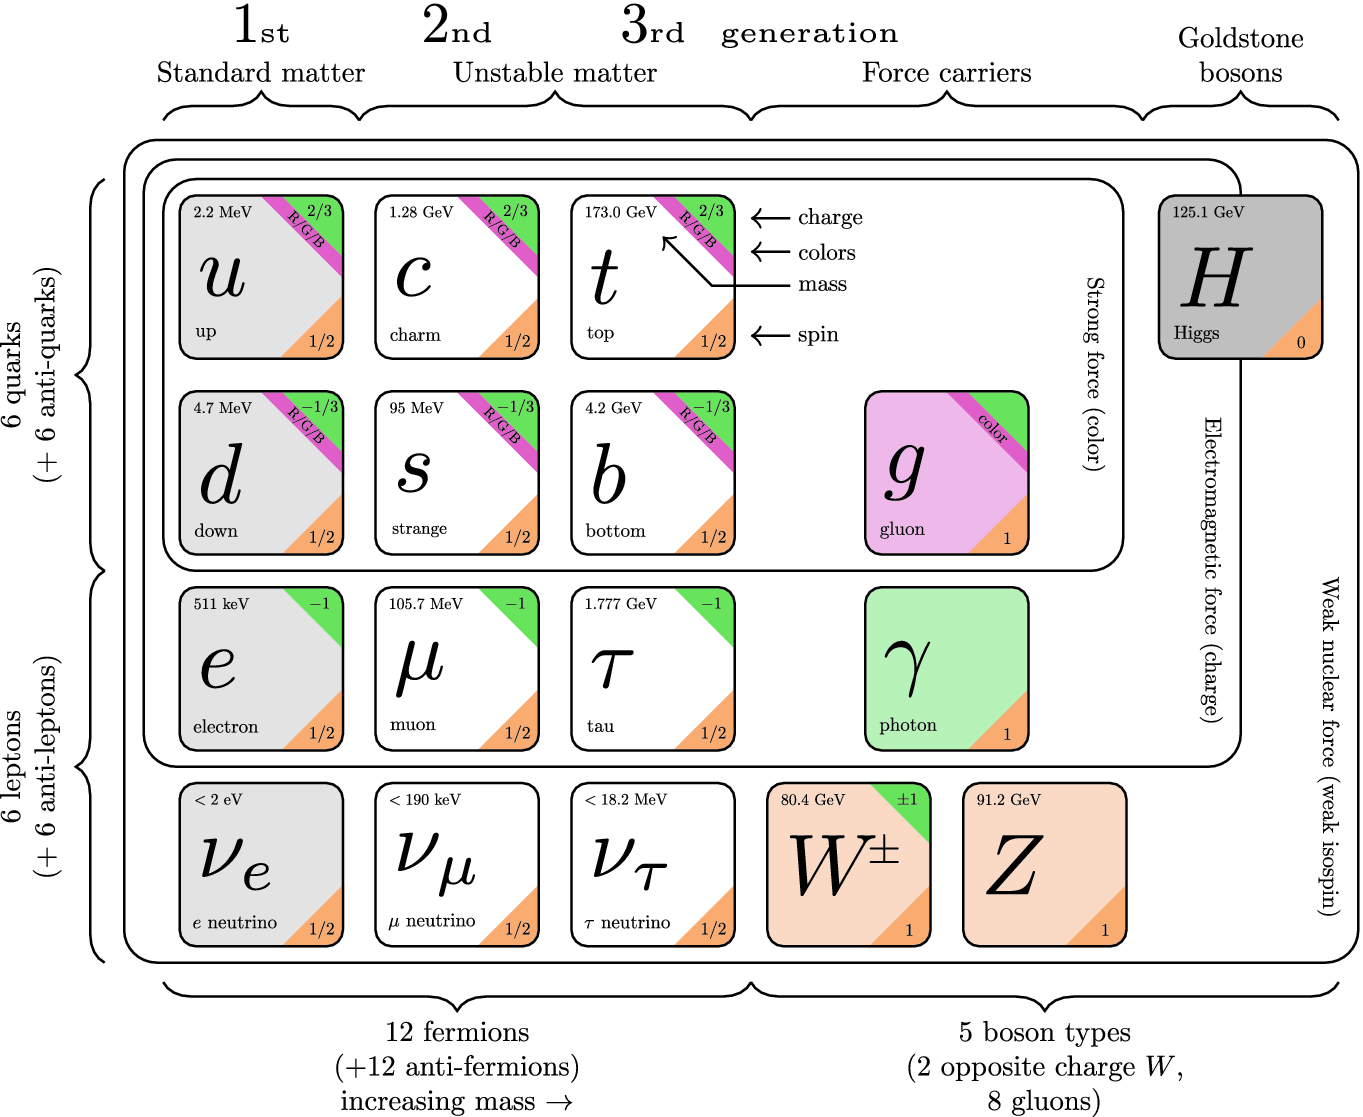
\includegraphics[width=5.2cm, height=4cm]{figs/SMFermions.png}
\end{center}
\end{figure} \vfill

However, this model \alert{has several shortcomings}: eventual exotic particles which do not fit within this model (such as dark matter) are extensively searched for nowadays. \vfill
\end{frame}

\begin{frame}{At the origins of dark matter I}
\justifying
The concept of dark matter can be traced back to the 19th century, and was introduced to \textbf{explain several astrophysical evidences}, among which: \vfill

\vspace{10pt}	
\begin{block}{ \centering Zwicky's calculations}\end{block}

\begin{itemize}
\justifying
\item Measurement of the mass of the Coma Cluster using the virial theorem;
\item Concluded that its mass was \textbf{400-500 times larger} than the value obtained by Hubble, considering only visible galaxies \cite{Zwicky}.
\end{itemize} \vfill

\vspace{10pt}	
\begin{block}{ \centering Spiral galaxies rotation curves}\end{block}

\begin{columns}
	\begin{column}{0.65\textwidth}
\begin{itemize}
\justifying
\vspace{-5pt}	
\item Stars within spiral galaxies should rotate with a velocity depending on the radius to the galactic center, but \textbf{this is not what is observed experimentally} \cite{RotationCurves};
\vspace{1pt}	
\item Either our understanding of gravity at large scales or our basic understanding of galaxies as a celestial body made of stars has to be revised.
\end{itemize} 
\end{column}

\begin{column}{0.44\textwidth}
\begin{figure}[htbp]
\begin{center}
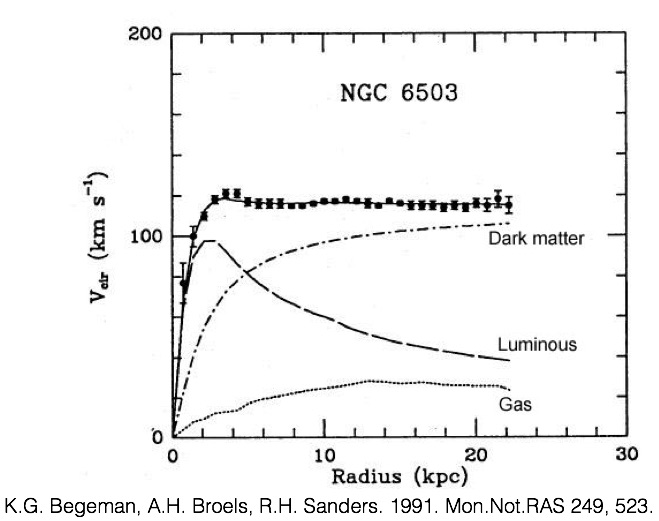
\includegraphics[width=4.5cm, height=3.7cm]{figs/RotationCurve.jpeg}
\end{center}
\end{figure}
\end{column}
\end{columns} \vfill

\end{frame}

\begin{frame}{At the origins of dark matter II}
\justifying

\vspace{5pt}
\begin{block}{ \centering CMB anisotropies}\end{block}

\begin{itemize}
\justifying
\item Background of primary radio waves emitted when the Universe became transparent around 380 000 years after the Big Bang;
\item Can be considered as emitting a black body spectrum with a temperature of $(2.72548\pm 0.00057)$K \cite{CMBTemperature}, but small anistropies at the $10^{-5}$ level are observed;
\item Implies that dark matter \alert{accounts for $\sim 27\%$ of the total mass of the Universe}.
\end{itemize} \vfill

\begin{columns}
	\begin{column}{0.54\textwidth}
\begin{figure}[htbp]
\begin{center}
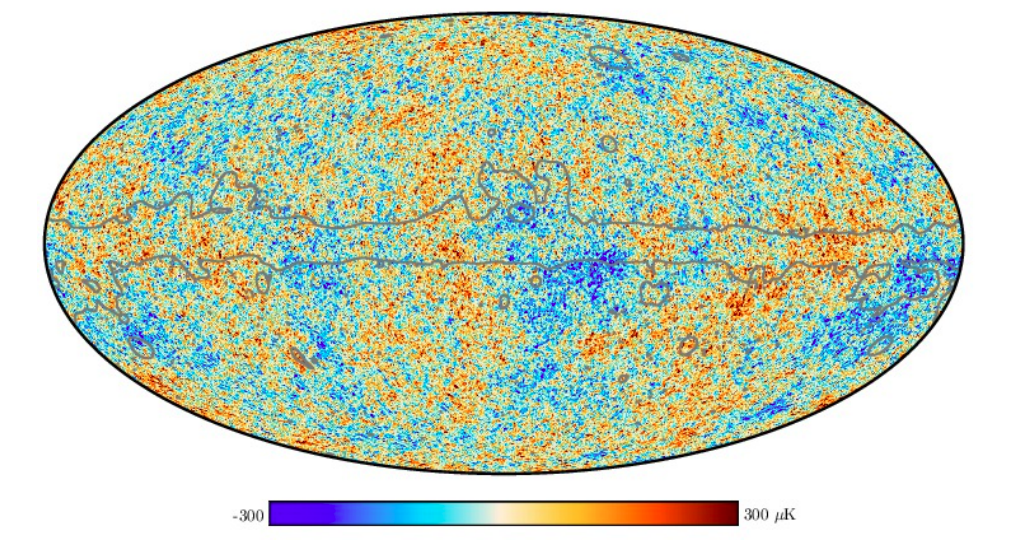
\includegraphics[width=6.5cm, height=3cm]{figs/PlanckTemperature.png}
\end{center}
\end{figure}
\end{column}
\begin{column}{0.44\textwidth}
\begin{figure}[htbp]
\begin{center}
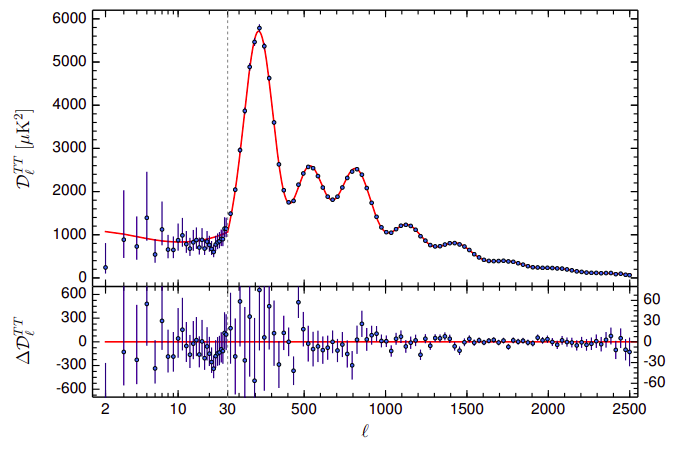
\includegraphics[width=5cm, height=3.5cm]{figs/PlanckSpectrum.png}
\end{center}
\end{figure}
\end{column}
\end{columns} \vfill

Other observations, such as the gravitational lensing effect, \textbf{also tend to further support the existence of dark matter} (cf. backup). \vfill
\end{frame}

\begin{frame}{Dark matter properties}
\justifying

\textbf{Several fundamental properties of dark matter} are nowadays known or assumed:

\begin{itemize}
\justifying
\item Dark matter \alert{is a particle}, given that it is assumed to have a certain mass;
\item It should be \alert{dark}, unable to interact with electromagnetic radation, otherwise we would have seen it already. It should then also be \textbf{electrically neutral};
\item It is \alert{non-baryonic}, because the energy density for the baryonic matter estimated from the CMB is too low to account for dark matter;
\item We only consider \alert{cold dark matter} since the widely accepted $\Lambda_{CDM}$ model is based on this assumption and this helps explaining the presence of large scale structures in the Universe;
\item It should \alert{have a mass in the electroweak scale}, between 10 GeV and 1 TeV, because of the relic density obtained from the thermal freeze-out mechanism \cite{Freezeout1}.
\item Finally, it should be \alert{long-lived}, since we expect them to have been produced during the Big Bang and they are still present in the Universe.
\end{itemize}

\end{frame}

\begin{frame}{Dark matter searches}
\justifying

\vspace{5pt}
\begin{block}{ \centering Weakly Interactive Massive Particles}\end{block} \vfill
The WIMPs are the dark matter candidates considered in this work, because of the so-called \textbf{WIMP miracle}. Indeed, they:

\begin{itemize}
\justifying
\item Are expected to interact very weakly with ordinary baryonic matter;
\item Have a mass in the 100 GeV-1 TeV range for reasonable electroweak production cross-section values;
\item Give us a dark matter while being able to solve the \textbf{hierarchy problem}.
\end{itemize} \vfill

\vspace{5pt}
\begin{block}{ \centering Search strategies}\end{block} \vfill

\begin{columns}
	\begin{column}{0.45\textwidth}
\begin{figure}[htbp]
\begin{center}
\begin{figure}[htbp]
\begin{center}
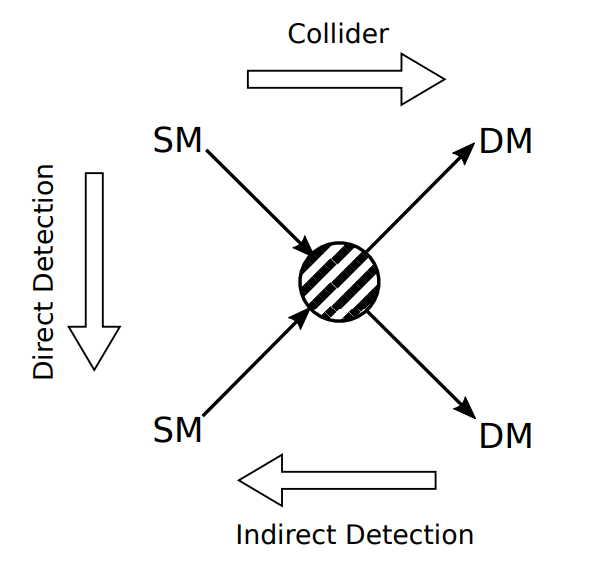
\includegraphics[width=4.2cm, height=3.5cm]{figs/ThreeWays.png}
\end{center}
\end{figure}
\end{center}
\end{figure}
\end{column}
\begin{column}{0.54\textwidth}
Different strategies are used:

\begin{itemize}
\justifying
\item The \textbf{direct and indirect searches}, relying on the production of baryonic
matter from the interaction between two DM particles or on the observation of the interaction
between the dark and baryonic sectors;
\item And the \textbf{collider production}, able to probe lower dark matter candidates masses.
\end{itemize}

\end{column}
\end{columns} \vfill
\end{frame}

\begin{frame}{Focus of this thesis}
\justifying
Yukawa
\end{frame}

\begin{frame}{Previous relevant results}
\justifying

\end{frame}










\begin{frame}[standout]
The experimental setup
\end{frame}

\begin{frame}{The Large Hadron Collider I}
\justifying

\end{frame}

\begin{frame}{The Large Hadron Collider II}
\justifying

\end{frame}

\begin{frame}{The CMS detector I}
\justifying

\end{frame}

\begin{frame}{The CMS detector II}
\justifying

\end{frame}












\begin{frame}[standout]
Analysis reminder
\end{frame}


\begin{frame}{Analysis reminder}
\justifying

Simplified model considered:

\begin{itemize} 
	\justifying
	\item Spin 1/2 DM $\chi$ ($\in [1, 55]$ GeV, Dirac fermion) \\
	\item Spin 0 scalar (S)/pseudoscalar (PS) mediator $\phi$ (Yukawa-like structure of such interactions $\rightarrow$ gain from the coupling of the mediator to top quarks) \\
	\item Mediator mass $\in [10, 1000]$ GeV \\
	\item Coupling $g_{\chi}$ mediator/DM set to 1 (same for all $g_q$ couplings) \\
	%\item Most samples cross-section at NLO
	%\item No mixing between $\phi$ and the SM Higgs boson
\end{itemize}\vfill

\begin{columns}
	\begin{column}{0.49\textwidth}
		\begin{center}
			\begin{block}{ \centering $t/ \bar t$+DM models}\end{block}	
			%\alert{\textbf{$t$ + DM models}} \\ \vspace{5pt}
			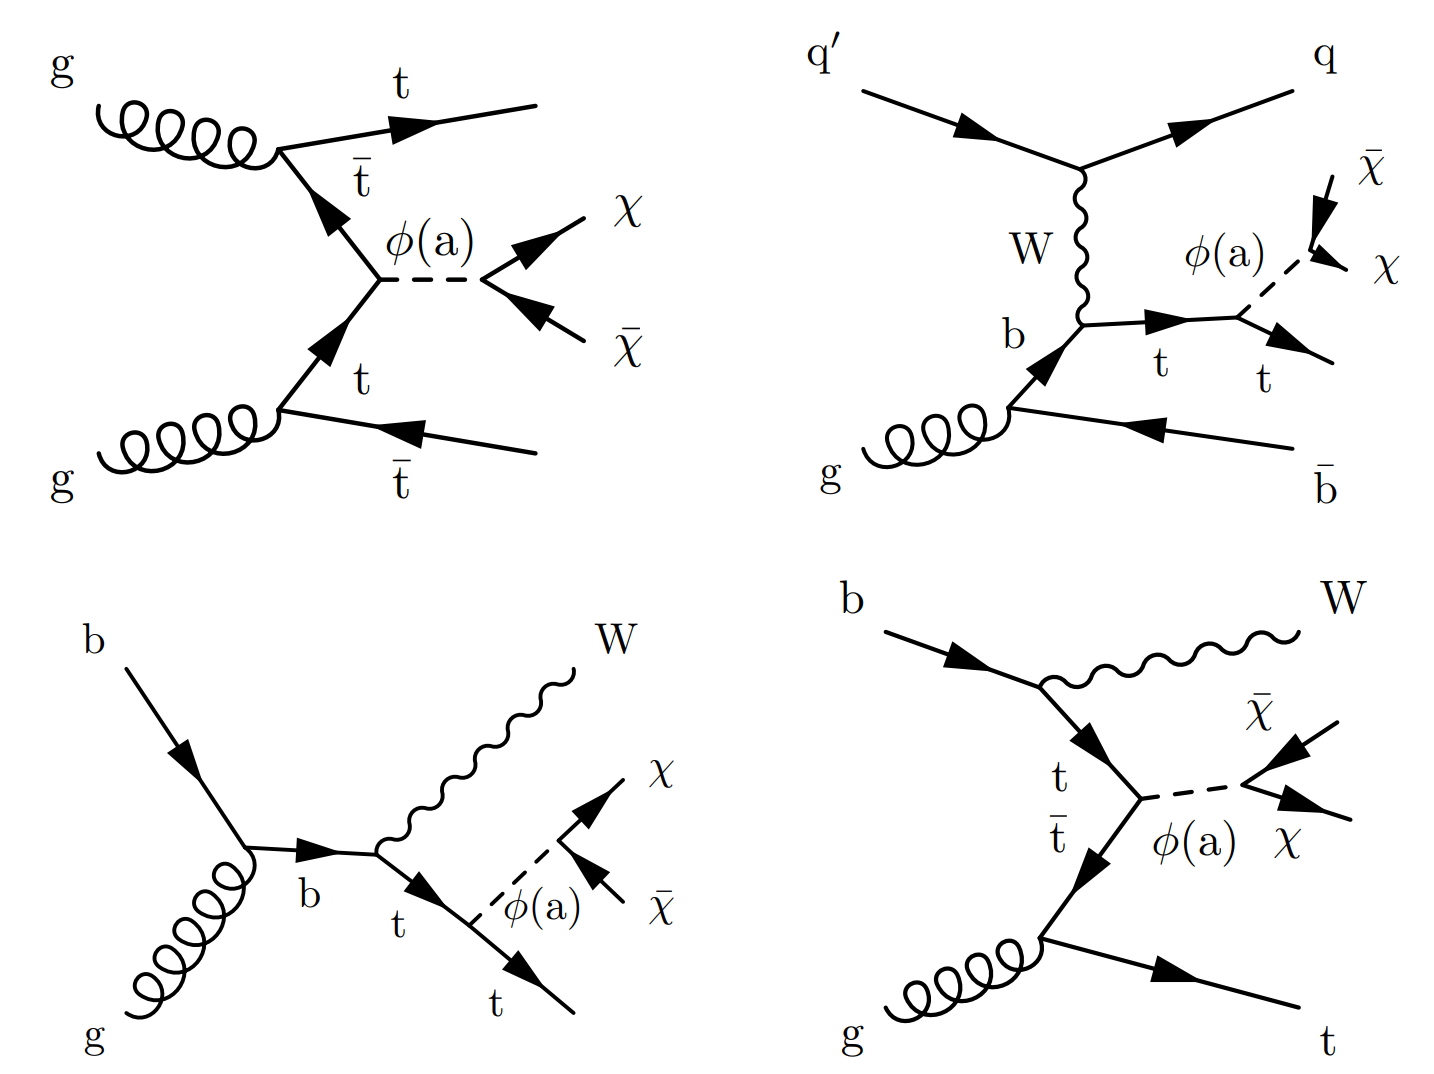
\includegraphics[width=0.8\textwidth]{figs/tDMfeynman.png}
    		 \end{center}
	\end{column} \hfill
	\begin{column}{0.49\textwidth}
		\begin{center}
			\begin{block}{\centering $t \bar t$+DM model}\end{block}				
			%\alert{\textbf{$t \bar t$ + DM model}} \\ \vspace{5pt}
			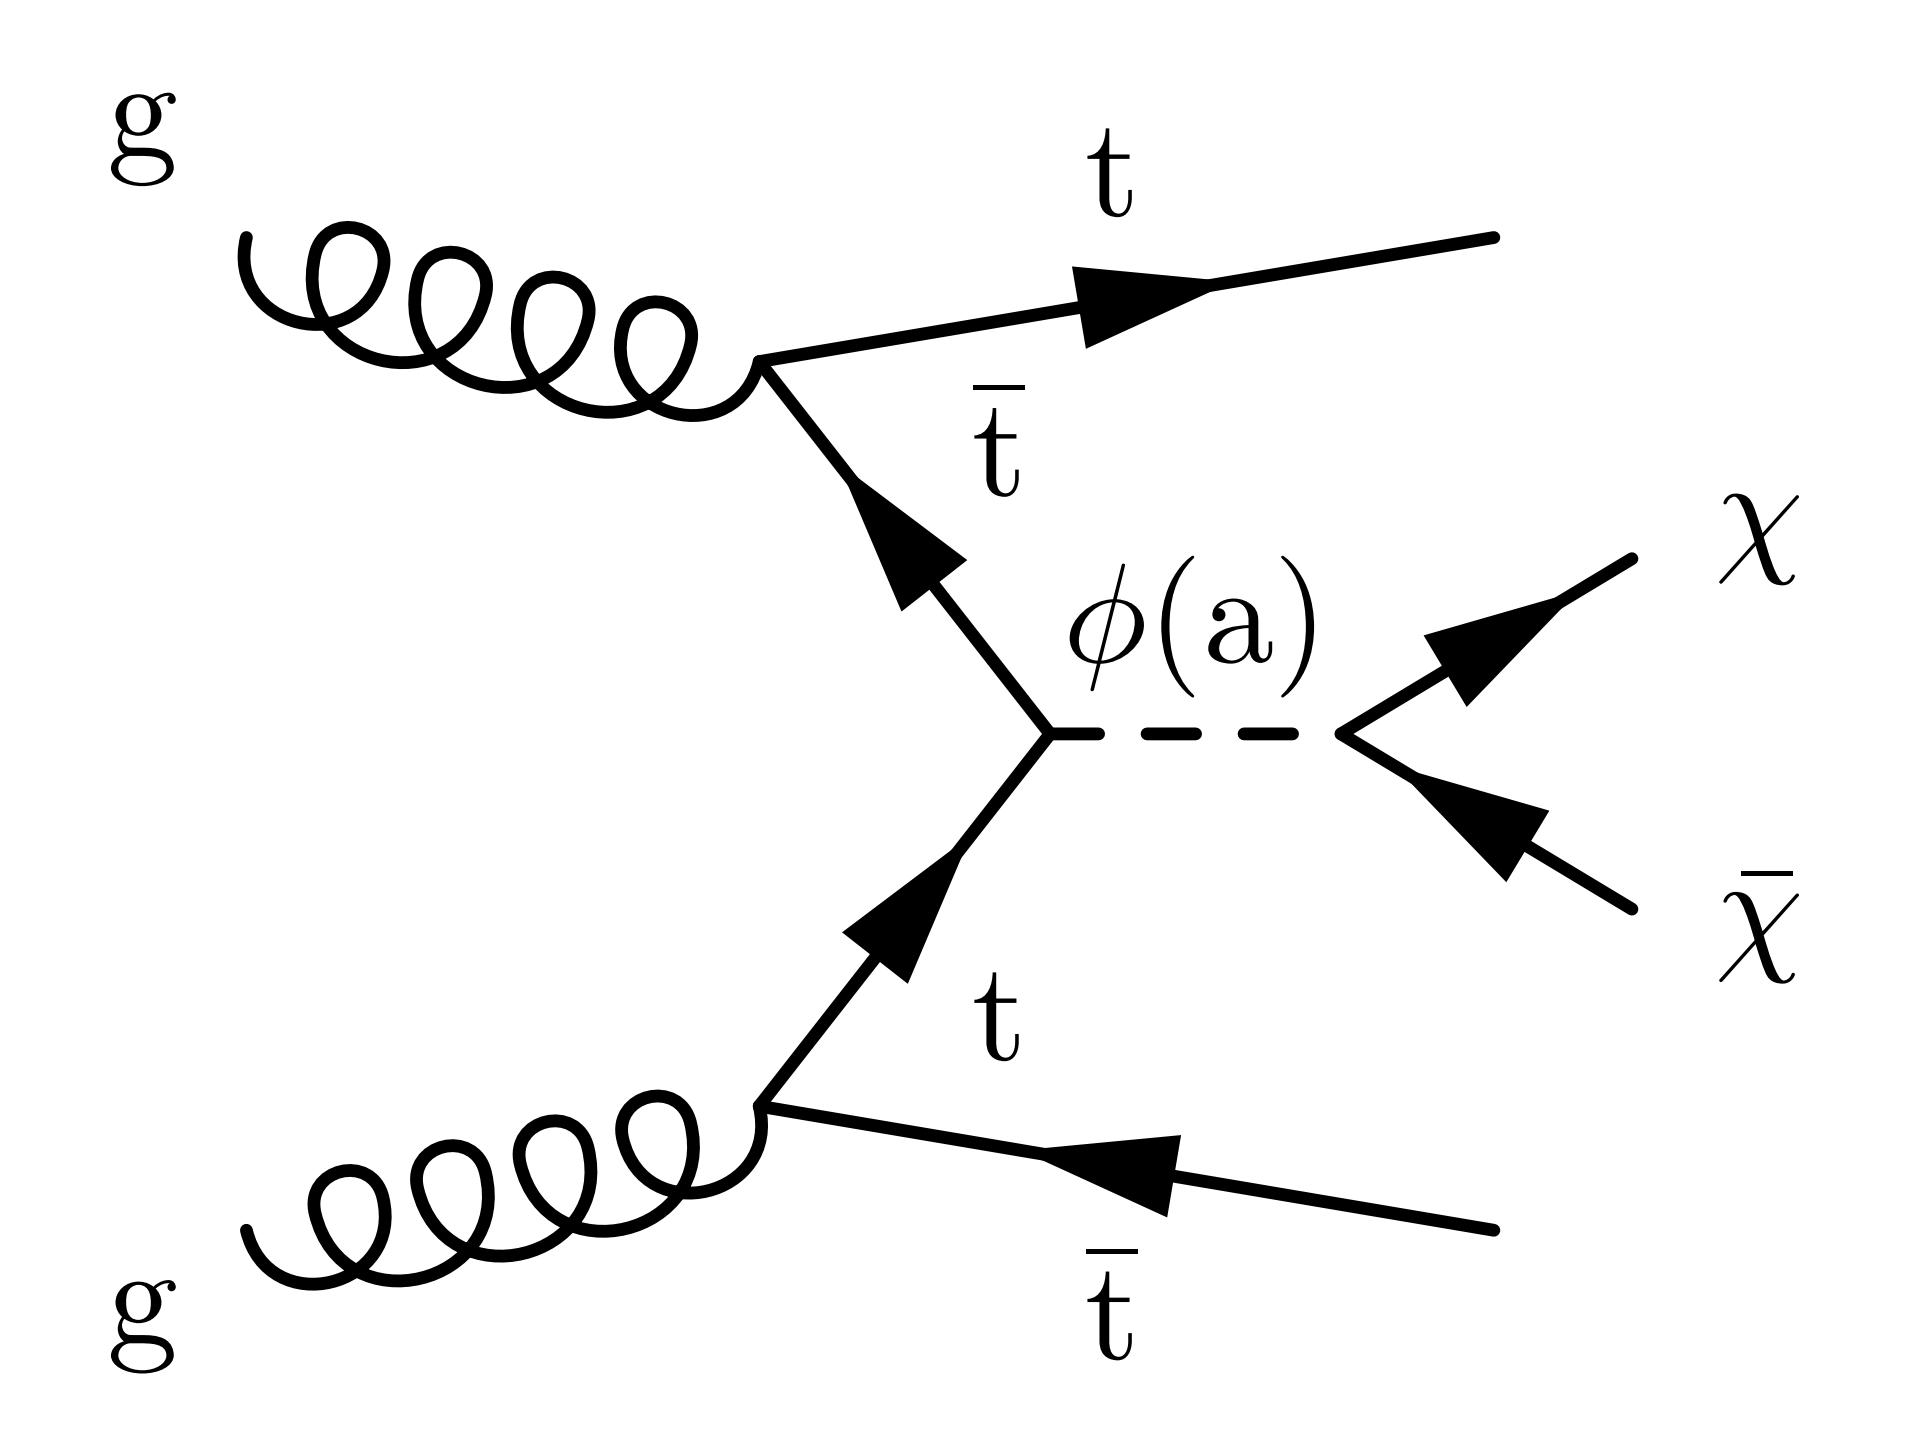
\includegraphics[width=0.80\textwidth]{figs/ttDM.png}
    		 \end{center}
	\end{column} \hfill
\end{columns} \vfill
\end{frame}

\begin{frame}{2016 results}
\justifying
The inclusion of the $t/ \bar t$+DM process \alert{improves up to a factor 2 } the limits obtained by the $t \bar t$ analysis on its own. Published in 2016 as \href{http://cms.cern.ch/iCMS/analysisadmin/cadilines?line=EXO-18-010&tp=an&id=2085&ancode=EXO-18-010}{\beamergotobutton{CMS-EXO-18-010}}.

\begin{itemize}
\item Only considering semi-leptonic and hadronic final states
\item Scalar (pseudoscalar) mediators \alert{excluded up to 290 (300) GeV} at 95\% CL.
%\item Usually lower production cross-section than the $t \bar t$ + DM (30-100\%)
%\item But non-flavour violating single top quark processes kinematically favored
\end{itemize} \vfill

\begin{center}
\begin{columns}
	\begin{column}{1.0\textwidth}
		\begin{center}
			%\begin{block}{\centering $t \bar t$+DM limits}\end{block}				
			%\alert{\textbf{$t \bar t$ + DM model}} \\ \vspace{5pt}
			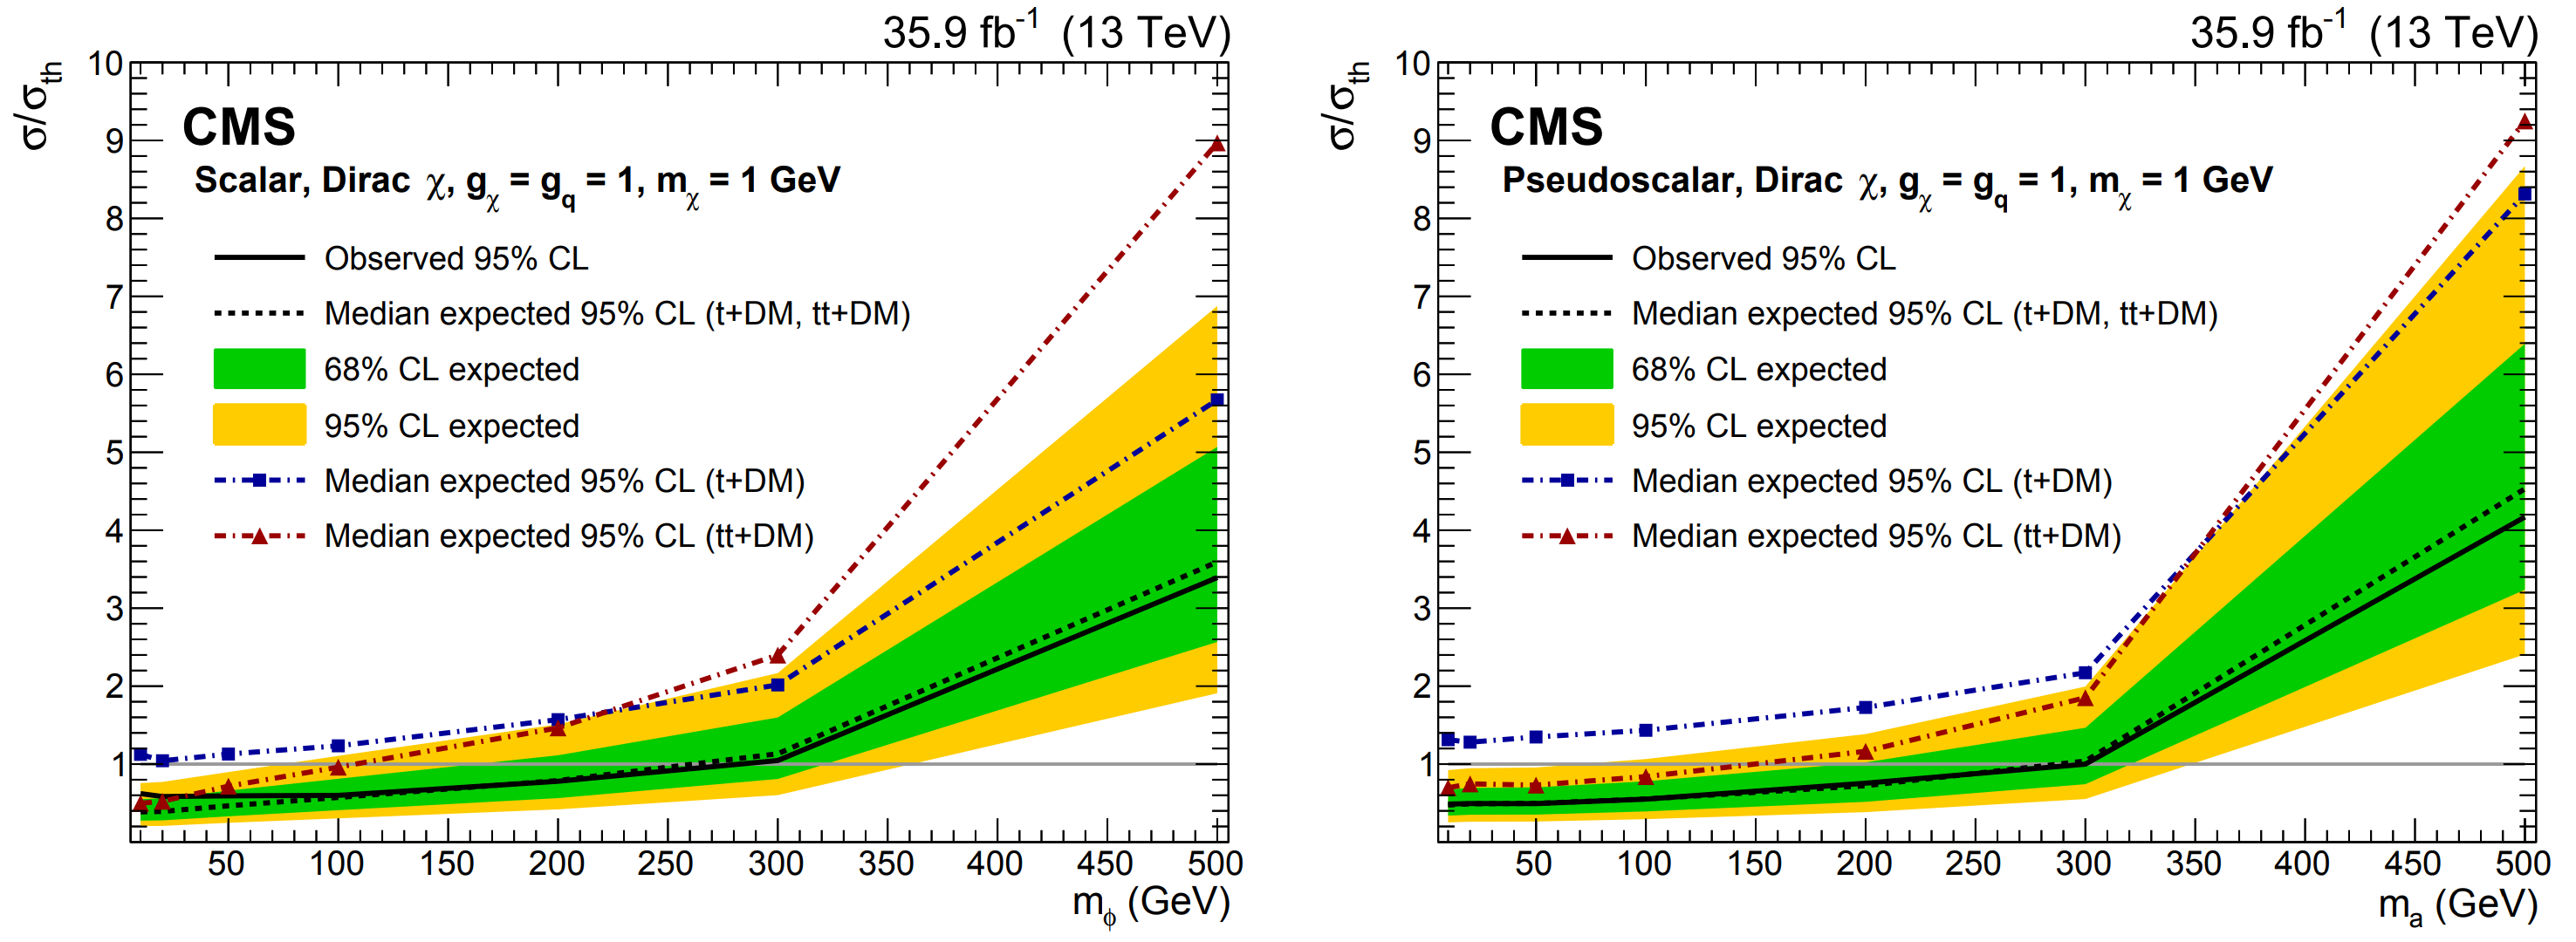
\includegraphics[width=1.0\textwidth]{figs/limitsprevious.png}
    		 \end{center}
	\end{column} \hfill
\end{columns} \vfill

\end{center} \vfill

\end{frame}

\begin{frame}{Analysis strategy}
\justifying
Run II legacy paper expected to \alert{combine both the $t$+DM and $t \bar t$+DM analyses}, and the 3 different final states (hadronic, one and two leptons). \vfill
This talk mostly focuses on:
\begin{itemize}
\justifying
\item Explaining the global strategy and status of the analysis 
\item Show the latest news and plans for each final state 
\item Display the two leptons final state latest distributions for 2016, 2017 and 2018
\end{itemize} \vfill
The effort is \alert{globally common} between the groups:
\begin{itemize}
\item Objects will be defined in a common way
\item Control and signal region orthogonal between the channels
\begin{itemize}
\item Number of leptons and b-jet categorization to improve the sensitivity by defining enriched single top/$t \bar t$ regions
\end{itemize}
\end{itemize}
\end{frame}

\begin{frame}[standout]
Dilepton final state
\end{frame}

\begin{frame}{Global strategy}
%\justifying
%The global strategy is to train a MVA (either BDT or DNN) to separate the two signals from the background, mainly the SM $t \bar t$ and the single top.
%
%To do this, a Multiclass method is currently used, teaching a single network to classify an event as either $t/\bar t$+DM, $t \bar t$+DM or background. \vfill

\begin{block}{\centering Frameworks}\end{block}
\alert{Two different frameworks} currently used in coordination:
\begin{itemize}
\justifying
\item Both frameworks use nanoAODv7 and the same samples
\item A synchronization exercise has been performed in the different control and signal regions, in 2016, 2017 and 2018, as documented in our twiki [1].
\end{itemize}
[1] \url{https://twiki.cern.ch/twiki/bin/view/CMS/TopPlusDMRunIILegacy} \vfill
\end{frame}

\begin{frame}{Conclusions}
\justifying

\end{frame}

\appendix
\backupbegin

\begin{frame}[standout]
Back up
\end{frame}

\begin{frame}{Gravitational lensing}
\justifying
\vspace{5pt}
Consequence of the general relativity: massive objects placed between distant sources and the observer should be able to \textbf{act as lenses and bend the light of the source}. \vfill

\begin{itemize}
\justifying
\item The deviation of the light is \textbf{proportional to the mass of the intermediate object}, giving us a way to measure its mass;
\item The mass distribution obtained has been compared to the luminous distribution of several galaxies, \alert{leading to $8\sigma$ discrepancies} \cite{BulletClusterSigma}.
\end{itemize} \vfill

\vspace{-5pt}
\begin{figure}[htbp]
\begin{center}
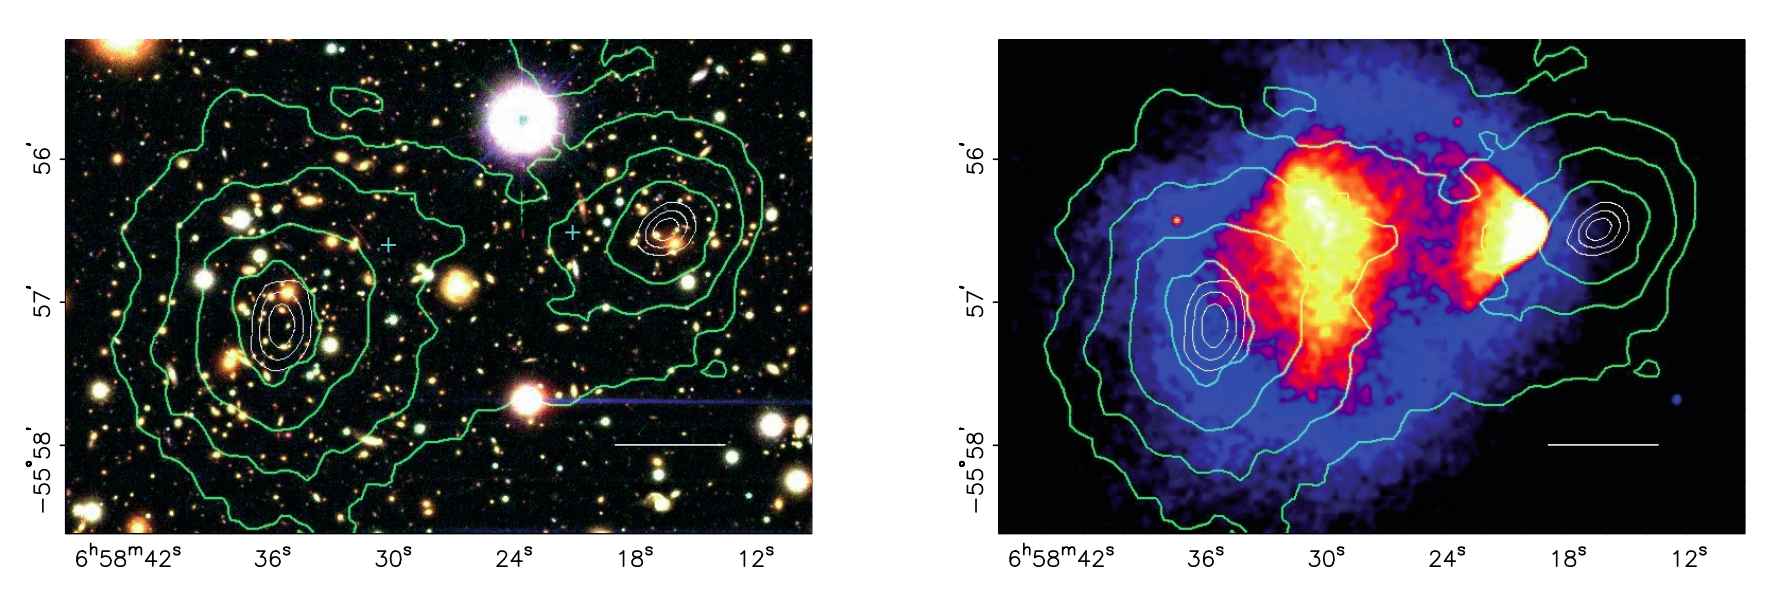
\includegraphics[width=11	cm, height=4cm]{figs/BulletCluster.png}
\end{center}
\end{figure} \vfill
\end{frame}

\begin{frame}{Thermal freeze-out}
\justifying
\vspace{5pt}
Schematic representation of the freeze-out process, representing the abundance of a
500 GeV dark matter with respect to the time and the impact of increasing cross-section annihilation
values on this freeze-out abundance. \vfill

\begin{figure}[htbp]
\begin{center}
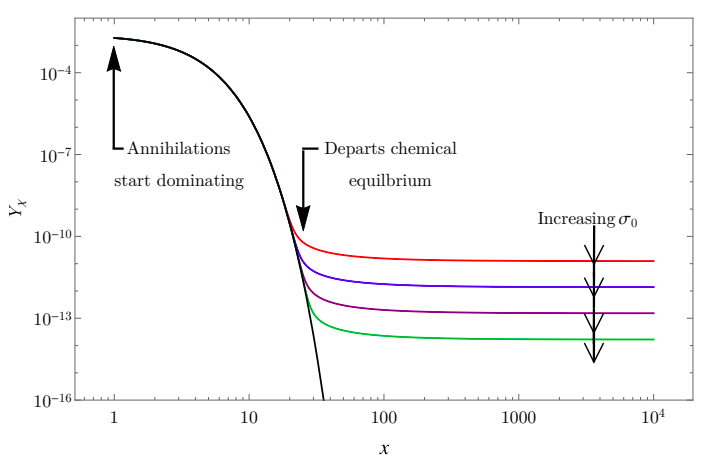
\includegraphics[width=9cm, height=6cm]{figs/FreezeOut.png}
\end{center}
\end{figure} \vfill
\end{frame}

\backupend

\begin{frame}{References}
\justifying

\begin{thebibliography}{1}
\bibitem{SMPredictions}
\href{https://arxiv.org/abs/1808.10518}{J. Woithe, G.J. Wiener and F. Van der Vecken,
"Let's have a coffee with the Standard Model of particle physics!",
Physics education 52, number 3, 2017
}

\bibitem{Zwicky} 
\href{http://articles.adsabs.harvard.edu/cgi-bin/nph-iarticle_query?1933AcHPh...6..110Z&amp;data_type=PDF_HIGH&amp;whole_paper=YES&amp;type=PRINTER&amp;filetype=.pdf}{
F. Zwicky,
"Die Rotverschiebung von extragalaktischen Nebeln",
Helvetica Physica Acta , vol. 6, pp. 110-127, 1933}

\bibitem{RotationCurves}
\href{https://academic.oup.com/mnras/article/249/3/523/1005565}{K.G. Begeman, A.H. Broeils and R.H. Sanders,
"Extended rotation curves of spiral galaxies - Dark haloes and modified dynamics",
Monthly Notices of the Royal Astronomical Society, vol. 249, issue 3, ISSN 0035-8711, 1991}

\bibitem{CMBTemperature}
\href{https://iopscience.iop.org/article/10.1088/0004-637X/707/2/916}{D.J. Fixsen,
"The temperature of the cosmic microwave background",
Astrophysical Journal, 2009
}

\bibitem{Freezeout1}
\href{https://arxiv.org/abs/1912.02828}{L. Heurtier, H. Partouche,
"Spontaneous Freeze Out of Dark Matter From an Early Thermal Phase Transition",
CPHT-RR065.112019 [arXiv: 1912.02828]}

\bibitem{BulletClusterSigma}
\href{https://iopscience.iop.org/article/10.1086/508162}{D. Clowe et all.,
"A Direct Empirical Proof of the Existence of Dark Matter",
Astrophysical Journal Letters 648, 2006
}
\end{thebibliography}
\end{frame}

\end{document}
